%%%%%%%%%%%%%%%%%%%%%%%%%%%%%%%%%%%%%%%%%%%%%%%%%%%%%%%%%%%%%%%%%%%%%%%%%%%%%%%%
%
% Plantilla para libro de texto de matemáticas.
%
% Esta plantilla ha sido desarrollada desde cero para el proyecto apuntesDGIIM
% de LibreIM.
%
%	Copyright (C) 2019 LibreIM
%
% This program is free software: you can redistribute it and/or modify
% it under the terms of the GNU Affero General Public License as
% published by the Free Software Foundation, either version 3 of the
% License, or (at your option) any later version.
% This program is distributed in the hope that it will be useful,
% but WITHOUT ANY WARRANTY; without even the implied warranty of
% MERCHANTABILITY or FITNESS FOR A PARTICULAR PURPOSE.  See the
% GNU Affero General Public License for more details.
% You should have received a copy of the GNU Affero General Public License
% along with this program.  If not, see <https://www.gnu.org/licenses/>.
%
%%%%%%%%%%%%%%%%%%%%%%%%%%%%%%%%%%%%%%%%%%%%%%%%%%%%%%%%%%%%%%%%%%%%%%%%%%%%%%%%

% ------------------------------------------------------------------------------
% CONFIGURACIÓN BÁSICA DEL DOCUMENTO
% ------------------------------------------------------------------------------

\documentclass[fontsize=12pt]{scrartcl}
\usepackage[spanish, es-tabla, es-lcroman, es-noquoting, es-minimal]{babel}
\usepackage{graphicx}

\usepackage{templatetools}

% ------------------------------------------------------------------------------
% CONFIGURACIÓN DE ASIGNATURA
% ------------------------------------------------------------------------------

\usepackage{config}

% ------------------------------------------------------------------------------
% TIPOGRAFÍA
% ------------------------------------------------------------------------------

% Tipografía personalizada
\usepackage[bitstream-charter]{mathdesign}
\usepackage[scale=0.88, type1]{FiraSans}
\usepackage[scale=0.88, type1]{FiraMono}
\usepackage[T1]{fontenc}

% Microtype
\usepackage[activate={true, nocompatibility}, final, tracking=true,factor=1100, stretch=10, shrink=10]{microtype}
\SetTracking{encoding={*}, shape=sc}{0}

% ------------------------------------------------------------------------------
% DISEÑO DE PÁGINA
% ------------------------------------------------------------------------------

% Márgenes
\usepackage[bottom=3.125cm, top=2.5cm, left=2.5cm, right=4.5cm, marginparwidth=70pt]{geometry}

% Párrafos
\linespread{1.1}
\setlength{\parindent}{12pt}
\setlength{\parskip}{0pt}

% Listas
\setlist{noitemsep}

% Cabeceras
\usepackage[automark]{scrlayer-scrpage}
\clearpairofpagestyles
\chead{\leftmark}
\cfoot*{\pagemark}

% Enlaces
\usepackage{hyperref}
\hypersetup{
	colorlinks=true,
	linkcolor=500,
}

% No mostrar cabecera en páginas de sección
\usepackage{xpatch}
\xpretocmd{\section}{\vspace*{1cm}\thispagestyle{plain}}{}{}

% Páginas de color para portada
\usepackage{pagecolor}
\usepackage{afterpage}

% ------------------------------------------------------------------------------
% ENTORNOS PERSONALIZADOS
% ------------------------------------------------------------------------------

\usepackage[theorems, skins, breakable]{tcolorbox}

\tcolorboxenvironment{nth}{
	blanker,
	breakable,
	left=12pt,
	before skip=12pt,
	after skip=12pt,
	borderline west={2pt}{0pt}{500},
	before upper={\parindent 12pt},
}

\tcolorboxenvironment{nprop}{
	blanker,
	breakable,
	left=12pt,
	before skip=12pt,
	after skip=12pt,
	borderline west={2pt}{0pt}{300},
	before upper={\parindent 12pt},
}

\tcolorboxenvironment{ncor}{
	blanker,
	breakable,
	left=12pt,
	before skip=12pt,
	after skip=12pt,
	borderline west={2pt}{0pt}{300},
	before upper={\parindent 12pt},
}

\tcolorboxenvironment{ndef}{
	skin=enhancedmiddle jigsaw,
	frame hidden,
	colback=50,
	breakable = true,
	break at = -6pt,
	top = 4pt,       % Estos márgenes están un poco a ojo
	bottom = 4pt,
	left= 8pt,
	right = 8pt,
	before skip=8pt, % Normalmente dejamos 12pt, pero
	after skip=8pt,  % aquí tenemos espacio adicional por el fondo
	no borderline,
	borderline west={2pt}{0pt}{500},
	borderline east={2pt}{0pt}{50},
	before upper={\parindent 12pt},
}

\tcolorboxenvironment{ejer}{
	skin=enhancedmiddle jigsaw,
	frame hidden,
	colback=50,
	breakable = true,
	break at = -6pt,
	top = 4pt,       % Estos márgenes están un poco a ojo
	bottom = 4pt,
	left= 8pt,
	right = 8pt,
	before skip=8pt, % Normalmente dejamos 12pt, pero
	after skip=8pt,  % aquí tenemos espacio adicional por el fondo
	no borderline,
	borderline west={2pt}{0pt}{500},
	borderline east={2pt}{0pt}{50},
	before upper={\parindent 12pt},
}

% ------------------------------------------------------------------------------
% LISTINGS
% ------------------------------------------------------------------------------

\IfPackageLoaded{listings}{
	\renewcommand{\lstlistingname}{Listado}

	\lstset{
		frame=lines,
		rulecolor=\color{black},
		framerule=1pt,
		numbers=left,
		belowcaptionskip=1\baselineskip,
		basicstyle=\ttfamily\color{black},
		keywordstyle=\bfseries\color{700},
		commentstyle=\color{300},
		stringstyle=\color{500},
		numberstyle=\color{black},
		breaklines=true,
		showstringspaces=false,
		tabsize=2,
	}
}

%%%%%%%%%%%%%%%%%%%%%%%%%%%%%%%%%%%%%%%%%%%%%%%%%%%%%%%%%%%%%%%%%%%%%%%%%%%%%%%%
% ------------------------------------------------------------------------------
% COMIENZO DEL DOCUMENTO
% ------------------------------------------------------------------------------
%%%%%%%%%%%%%%%%%%%%%%%%%%%%%%%%%%%%%%%%%%%%%%%%%%%%%%%%%%%%%%%%%%%%%%%%%%%%%%%%

\begin{document}

% ---------------------------------------------------------------------------
% PORTADA EXTERIOR
% ---------------------------------------------------------------------------

\newpagecolor{500}
\begin{titlepage}
	\noindent
	\setlength\fboxsep{0cm}
	\parbox[t]{\textwidth}{
			\raggedright
			\fontsize{50pt}{50pt}\selectfont\sffamily\color{white}{
			  \textbf{\asignatura}
      }
	}

	\vfill

	\noindent
	\parbox[b]{\textwidth}{
		\raggedright
		\sffamily\large\color{white}
		{\Large \autor }\\[4pt]
		\grado\\
		\universidad\\[4pt]
		\texttt{\enlaceweb}
	}

\end{titlepage}
\restorepagecolor

% ---------------------------------------------------------------------------
% PÁGINA DE LICENCIA
% ---------------------------------------------------------------------------

\thispagestyle{empty}
\null
\vfill

\noindent
\parbox[b]{0.7\textwidth}{
  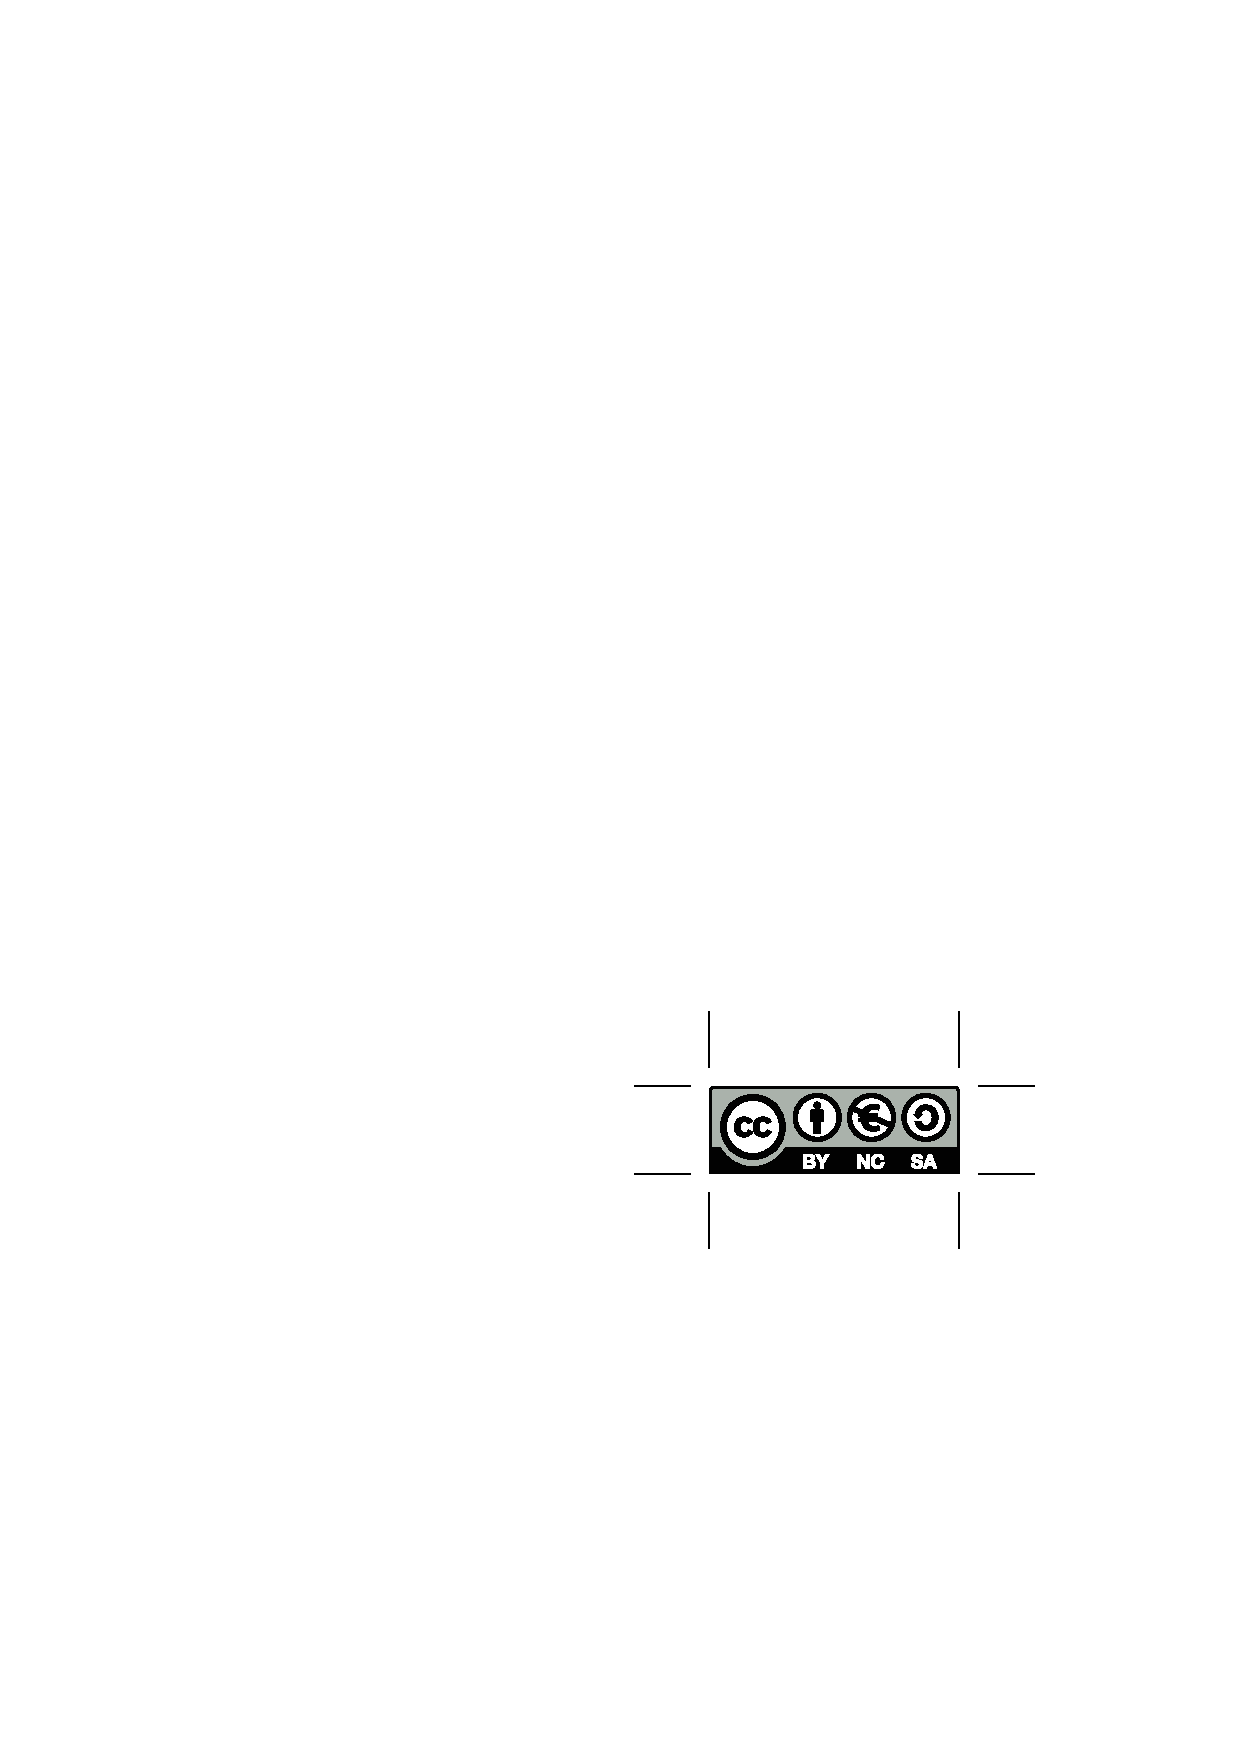
\includegraphics{by-nc-sa.pdf}\\[4pt]
  \raggedright
  \sffamily
  {\large Este libro se distribuye bajo una licencia CC BY-NC-SA 4.0.}\\[4pt]
  Eres libre de distribuir y adaptar el material siempre que reconozcas a los autores originales del documento, no lo utilices para fines comerciales y lo distribuyas bajo la misma licencia.\\[4pt]
  \texttt{creativecommons.org/licenses/by-nc-sa/4.0/}
}

% ---------------------------------------------------------------------------
% PORTADA INTERIOR
% ---------------------------------------------------------------------------

\begin{titlepage}

	\noindent
	\parbox[t]{\textwidth}{
			\raggedright
			\fontsize{50pt}{50pt}\selectfont\sffamily\color{500}{
			  \textbf{\asignatura}
      }
	}

	\vfill

	\noindent
	\parbox[b]{\textwidth}{
		\raggedright
		\sffamily\large
		{\Large \autor}\\[4pt]
		\grado\\
		\universidad\\[4pt]
		\texttt{\enlaceweb}
	}

\end{titlepage}

% ---------------------------------------------------------------------------
% ÍNDICE
% ---------------------------------------------------------------------------

\thispagestyle{empty}
{\hypersetup{linkcolor=black}\tableofcontents}
\newpage

% ---------------------------------------------------------------------------
% CONTENIDO
% ---------------------------------------------------------------------------

\part{Teoría}
\section{Fundamentación probabilística de vectores aleatorios}

\begin{ndef}[Variable Aleatoria]
    Sea $(\Omega, \mathcal{F}, P)$ un espacio de probabilidad. Una \textit{variable aleatoria} es una función medible
    \begin{align*}
    X:(\Omega, \mathcal{F}) &\rightarrow (\mathbb{R}, \mathbb{B})\\
    \omega &\mapsto X(\omega)
    \end{align*}
    cuya condición de medibilidad es \(X^{-1}(B) \in \mathcal{F}\) para todo \(B \in \mathbb{B}\).
\end{ndef}

\begin{ndef}[Probabilidad inducida]
    La \textit{probabilidad inducida} por una variable aleatoria $X$ a partir de $P$ se define como
    \begin{align*}
    P_{X}:\mathbb{B} &\rightarrow [0,1] \\
    B &\mapsto P[X^{-1}(B)].
    \end{align*}
\end{ndef}

\begin{ndef}[Vector Aleatorio]
    Sea $(\Omega, \mathcal{F}, P)$ un espacio de probabilidad. Un \textit{vector aleatorio}, $\boldsymbol X = (X_1, \dots, X_p)$ es una función medible
    \begin{align*}
      \boldsymbol X:(\Omega, \mathcal{F}) &\rightarrow (\mathbb{R}^p, \mathbb{B}^p) \\
    \omega &\mapsto \boldsymbol X(\omega) = (X_1(\omega), \dots, X_p(\omega))
    \end{align*}
    cuya condición de medibilidad es \(\boldsymbol X^{-1}(B) \in \mathcal{F}\) para todo \( B \in \mathbb{B}^p\).
\end{ndef}

\begin{ndef}[Probabilidad inducida]
    La \textit{probabilidad inducida} por un vector aleatorio $\boldsymbol X = (X_1, \dots, X_p)$ a partir de $P$ se define como
    \[
    P_{\boldsymbol X}[B] := P[\boldsymbol X^{-1}(B)]
    .\] para todo \(B \in \mathbb{B}^p\).
\end{ndef}

\begin{ndef}[Función de distribución]
    Se define la \textit{función de distribución} asociada a $P_{\boldsymbol X}$ como
    \begin{align*}
    F_{\boldsymbol X}:\mathbb{R}^p &\rightarrow [0,1] \\
    \boldsymbol x=(x_1,\dots,x_p) &\mapsto P_{\boldsymbol X}[X_1 \leq x_1, \dots, X_p \leq x_p]\,.
    \end{align*}
\end{ndef}

\begin{ndef}[Función de densidad]
    Si existe una función $f_X$ que sea integrable en el sentido de Lebesgue y tal que
    \[
    F_{\boldsymbol X}(x) = \int^{x_1}_{-\infty} \dots \int^{x_p}_{-\infty} f_{\boldsymbol X}(u_1, \dots,  u_p) \mathop{}\!\mathrm{d}u_1 \dots \mathop{}\!\mathrm{d}u_p \quad \text{para todo } \boldsymbol  x \in \mathbb{R}^p
    ,\]
    diremos que $f_{\boldsymbol X}$ es la \textit{función de densidad} asociada a  $F_{\boldsymbol X}$. En el caso en que $f_{\boldsymbol X}$ sea continua, se puede escribir como:
    \[
    % TODO Añadir lo de las derivadas
    f_{\boldsymbol X}(\boldsymbol x) = \frac{\partial^p}{\partial x_1 \dots \partial x_p} F_{\boldsymbol X}(\boldsymbol x) \quad \text{para todo } \boldsymbol x \in \mathbb{R}^p
    .\]
\end{ndef}

En general, dado un conjunto producto (también llamado conjunto rectangular) $B \in \mathbb{B}^p$ con
\[
    B = B_1 \times \dots \times B_p,\quad B_j \in \mathbb{B}, \quad j = 1, \dots, p
.\]
se tiene que
\[
P_{\boldsymbol X}[B] \neq P_{X_1}[B_1] \dots  P_{X_p}[B_p].
\]

\begin{ndef}
    Si en las condiciones anteriores se da la igualdad para todo conjunto producto en \(\mathbb{B}^p\), se dice que \(X_1, \dots, X_p\) son \textit{independientes}.

    Equivalentemente, esto ocurre si y solo si \(
    F_{\boldsymbol X} (\boldsymbol x) = F_{X_1} (x_1) \cdots F_{X_p}(x_p)\,\) para todo \(\boldsymbol x \in \mathbb{R}^p\).

    Por último, esto ocurre en el caso continuo si y solo si \(f_{\boldsymbol X} (\boldsymbol x) = f_{X_1}(x_1) \cdots f_{X_p}(x_p)\,\) para todo \(\boldsymbol x \in \mathbb{R}^p\), salvo, a lo sumo, en un conjunto de medida de Lebesgue nula.
\end{ndef}

\subsection{Función característica}

\begin{ndef}[Función característica]
    La \textit{función característica} de un vector aleatorio \(\boldsymbol X = (X_1,\dots,X_p)\) se define como \[\psi_{\boldsymbol X}(\boldsymbol t)=E\left[e^{i\boldsymbol t^T\boldsymbol X}\right], \quad \boldsymbol t\in \mathbb{R}^p.\]
\end{ndef}

\begin{nth}[Unicidad]
  La función característica de un vector aleatorio determina de forma única su distribución.
\end{nth}

\begin{nprop}
  Las componentes de \(\boldsymbol X=(X_1,\dots,X_p)^T\) son independientes si, y solo si \[\psi_{\boldsymbol X}(\boldsymbol t)=E\left[e^{i\boldsymbol t^T\boldsymbol X}\right] = \prod_{k=1}^p\psi_{X_k}(t_k)\,.\]
\end{nprop}

\begin{nprop}
  Si las componentes de \(\boldsymbol X=(X_1,\dots, X_p)\) son independientes, entonces la función característica de la variable \(\boldsymbol Y=\sum_{k=1}^p X_k\) es \[\psi_{\boldsymbol Y}(\boldsymbol t)=E\left[e^{i\boldsymbol t^T\boldsymbol Y}\right] = \prod_{k=1}^p\psi_{X_k}(t).\]
\end{nprop}

\subsubsection{Transformaciones lineales}

Sea $\boldsymbol X = (X_1, \dots X_p)^T$ un vector aleatorio $p-$dimensional y sea $\boldsymbol Y = (Y_1,\dots,Y_q)^T$ otro vector aleatorio $q-$dimensional definido como
\[
  \boldsymbol Y = B\boldsymbol X + \boldsymbol b\,,
\]
con $B \in M_{qxp}$ una matriz constante y $\boldsymbol b\in \mathbb R ^n$.

\begin{nprop}
  La función característica de $\boldsymbol Y$ se obtiene como:
  \[
  \psi_{\boldsymbol Y}(\boldsymbol t) = E\left[e^{i\boldsymbol t^T \boldsymbol Y}\right] = \dots = e^{i\boldsymbol t^T \boldsymbol b} \psi_{\boldsymbol X}(B^T \boldsymbol t)\,, \quad \boldsymbol t = (t_1,\dots,t_q)^T \in \mathbb R^q\,.
  \]
\end{nprop}
%#TODO: escribir la forma matricial
%#TODO: ¿Está amsmath incluido? Usar bmatrix de amsmath
  En particular, si $\boldsymbol X= \left( X_{(1)}^T | X_{(2)}^T\right)^T$, $X=$ = ¡¡¡MATRIZ DE ARRIBA $X_1$ y abajo $X_2$!!!, con $X_{(1)}$ de dimensión $(k\times1)$ y $X_{(2)}$ de dimensión $(p-k) \times 1$, se tendría:
  \[
X_{(1)} = ( I_{k\times k} | O_{k \times(p-k)})X + O_{k\times 1}
\]
por lo que, para $\boldsymbol t_{(1)} = (t_1,\dots,t_k)^T \in \mathbb R^k$
\[
\psi_{X_{(1)}}\left(t_{(1)}\right) = e^{it^T 0} \psi_X\left(\frac{I_{k\times k}}{0_{k\times(p-k)}}\right) = \psi_X\left(\frac{t}{0_{(p-k)\times1}}\right)\,.
\]

\subsubsection{Relación con la función de densidad}

La función de densidad (en el caso continuo) de un vector aleatorio $\boldsymbol X = (X_1,\dots,X_p)^T$ y la correspondiente función característica constituyen un par de \emph{transformadas de Fourier}, de forma que
\[
\psi_{\boldsymbol X}(\boldsymbol t) = \int_{\mathbb R ^p} e^{i \boldsymbol t^T x} f_X(x) \mathop{}\!\mathrm{d}x\,,
\]
y por otro lado
\[
f_{\boldsymbol X}(x) =  \dfrac{1}{(2\Pi)^p} \int_{\mathbb R^p} e^{- i \boldsymbol t^T x} \psi_{\boldsymbol X}(t) \mathop{}\!\mathrm{d}t\,.
\]


\subsection{Aspectos generales sobre vectores aleatorios}
\subsubsection{Esperanza y covarianza}
\begin{ndef}
  Sea $\boldsymbol X=(X_1,\dots,X_n)^T$ un vector aleatorio. Se define el \textit{vector de medias} de $\boldsymbol X$ como:
  \[
  \boldsymbol \mu_{\boldsymbol X} = E[\boldsymbol X] = \begin{bmatrix}  E[X_1] \\ \dots \\ E[X_p] \end{bmatrix} = \begin{bmatrix} \mu_1 \\ \dots \\ \mu_p \end{bmatrix}
  \]
  Siempre que existan \emph{todas} las esperanzas unidimensionales
  \end{ndef}

\begin{nprop}[Propiedad de linealidad]
  Sea $\boldsymbol Y = B\boldsymbol X + \boldsymbol b$ con $B \in M_{q\times p}$ constante y $\boldsymbol b \in \mathbb R^q$ constante. Entonces,
  \[
    \boldsymbol \mu_{\boldsymbol Y} = E[\boldsymbol Y] = BE[\boldsymbol X] + \boldsymbol b = B\boldsymbol \mu_{\boldsymbol X} + \boldsymbol b\,.
\]
\end{nprop}
%#TODO: Demostración(ejercicio)

Podemos extender esta propiedad al caso de matrices aleatorias. Sea $X\in \mathcal M_{p\times q}$ es una matriz aleatoria, y $B\in \mathcal M_{m\times p}$ , $C \in \mathcal M_{q\times n}$ , $D \in \mathcal M_{m \times n}$ matrices constantes. Entonces, para $W = BXC + D$, una matriz aleatoria de dimensión $m\times n$, la matriz de medias viene dada por
\[
E[W] = \left(E[W_{kl}]\right)_{(kl)} = B \cdot E[X] \cdot C + D\,, \quad \text{con } E[X] = \left(E[X_{ij}]\right)_{(ij)}\,.
\]

\begin{ndef}
  Se define la \textit{matriz de covarianzas} del vector $\boldsymbol X = (X_1,\dots,X_p)^T$ como:
  \[
\Sigma = \operatorname{Cov}(\boldsymbol X) = E\left[(\boldsymbol X-\boldsymbol \mu)(\boldsymbol X-\boldsymbol \mu)^T\right] = \begin{bmatrix} \sigma_{11} & \dots & \sigma_{1p} \\ \vdots& \ddots & \vdots \\ \sigma_{p1} &  \dots & \sigma_{pp}\end{bmatrix}\,,
\]
con $\sigma_{ij} = E\left[(X_i - \mu_i)(X_j - \mu_j)\right] = \sigma_{ji}$. Solo puede definirse si existen todas las esperanzas. 
\end{ndef}

\begin{nota}
  Los elementos de la diagonal de la matriz de covarianzas se pueden calcular como \[\sigma_{ii}=E\left[(X_i - \mu_i)^2\right] = \operatorname{Var}(X_i) = \sigma_i^2\,,\]siendo $\sigma_i$ la \textit{desviación típica}.
\end{nota}

\begin{nprop}[Propiedades elementales]
  La matriz de covarianzas verifica las siguientes propiedades elementales:
  \begin{enumerate}
    \item Es simétrica.
    \item Los elementos de su diagonal son no negativos.
    \item La clase de matrices de covarianzas en dimensión $p\times p$ coincide con la clase de matrices simétricas definidas no negativas.
    \end{enumerate}
  \end{nprop}
%#TODO: demostración (Ejercicio)
\begin{proof}
  Vamos a ver únicamente la demostración de la propiedad 3.
  \begin{itemize}
    \item[3.] $\boxed{\implies}\,$ Supongamos que $\Sigma$ es la matriz de covarianza de un vector aleatorio $\boldsymbol X$, y $\boldsymbol \mu_{\boldsymbol X}$ es su vector de medias. Sea $\boldsymbol \alpha \in \mathbb R^p$. Tenemos que probar que $\boldsymbol \alpha^T \Sigma \boldsymbol \alpha^T \geq 0$. Consideramos la variable aleatoria $\boldsymbol \alpha^T \boldsymbol X$. \begin{align*}
      0 \leq Var(\alpha^T X) = E[(\alpha^T X - E[\alpha^T X])^2] &= E[(\alpha^T X - \alpha^T \mu_X)^2] = E[(\alpha^T(X-\mu)^2]\\ 
        &=^{(1)} E[\alpha^T(X-\mu)(X-\mu)^T \alpha] \\
        &= \alpha^T E[(X-\mu)(X-\mu)^T] \alpha \\
        &= \alpha^T \Sigma \alpha
    \end{align*} Donde en 1 hemos separado el cuadrado y hemos traspuesto uno de los términos (el resultado es el mismo, un escalar).

  $\boxed{\impliedby}\,$ Sea $\Sigma$ una matriz simétrica, definida no negativa. Sea $r = \operatorname{rango}(\Sigma)$ con $r\leq p$. Entonces, se puede encontrar $\Sigma = C C^T$. donde $C \in M_{p\times r}$. Sea... TERMINAR!

%#TODO: Terminar demostración
  \end{itemize}
\end{proof}

%#TODO: revisar el estilo de esta parte, quizá añadir una subsección?
Vamos a ver ahora diferentes \textbf{casos} que se pueden dar respecto a la matriz $\Sigma$.

\paragraph{Si $\Sigma$ es definida positiva} Se nota como $\Sigma > 0$. En este caso $\Sigma$ es \textit{no singular} pues $(|\Sigma| > 0)$, y por tanto existe su inversa, $\Sigma^{-1}$. Esto es interesante pues nos permite normalizar el vector aleatorio de manera que tenga un vector de medias cero y una matriz de covarianzas que sea la identidad.

\begin{nota}
  Usaremos la notación $X\sim(\mu,\Sigma)$ para denotar que la media y la matriz de covarianzas están bien definidas.
\end{nota}

\begin{ndef}[Normalización]
    Dado un vector aleatorio $\boldsymbol X\sim(\mu,\Sigma)$, con $\Sigma>0$, se define su \textit{normalización} en «origen» y «escala» como
    \[
  Z = C^{-1}(X - \mu)\,,
\]
para cualquier matriz $C\in M_{p\times p}$ tal que $E = CC^T$. Esta matriz $C$ no es única, pues existen infinitas descomposiciones de $\Sigma$ de esta forma.

  \end{ndef}

Veamos a continuación algunas de las propiedades de esta variable $Z$.
  \begin{itemize}
    \item
  $
  E[Z] = E[C^{-1}(X-\mu)] = C^{-1}E[(X-\mu)] = C^{-1}(E[X] - \mu) = C^{-1}(\mu - \mu ) = 0
  $

\item $\operatorname{Cov}(Z) = E[ZZ ^T] = E[C^{-1}(X-\mu)(X-\mu)^T(C^{-1})^T]$ y, por la propiedad de las matrices que nos dice que $(C^{-1})^T = (C^T)^{-1}$, se tiene en la igualdad anterior : $\operatorname{Cov}(Z) = C^{-1}E[(X-\mu)(X-\mu)^T](C^T)^{-1} = C^{-1} \Sigma (C^T)^{-1} = C^{-1}CC^T(C^T)^{-1} = I \cdot I = I \implies Z \sim (0, I_{p\times p}).$

  \end{itemize}

  \begin{ndef}
    Se define la \textit{distancia de Mahalanobis} de $X\sim(\mu,\Sigma)$ con $\Sigma > 0$ con respecto a su vector de medias como
    \[
    \Delta(X,\mu) = \left\{ (X-\mu)^T \Sigma (X-\mu) \right\} ^{\frac{1}{2}},
    \]
    que es una variable aleatoria.
  \end{ndef}

  Vamos a interpretar este resultado. Supongamos que tenemos una normalización de $X$:
  \[
  \Delta(X,\mu) = \left\{ (X-\mu)^T (CC^T)^{-1}(X-\mu)\right\}^{\frac{1}{2}} = \left\{ (X-\mu)^T (C^T)^{-1}C^{-1}(X-\mu)\right\}^{\frac{1}{2}} = \left\{Z^T Z\right\}^{\frac{1}{2}} = \Vert Z\Vert\,,
  \]
  con norma la euclídea en $\mathbb R^p$. Así, hemos relacionado la distancia con la norma. Recordemos que $\Vert Z\Vert$ es una variable aleatoria, pues es una aplicación de una función a un vector aleatorio.

  \begin{nprop}
    \begin{itemize}
    \item Calcular $E[\Delta^2 (X,\mu)]$
    \item La ecuación $\Delta(X,\mu) = k$ pcon $k\geq 0$ constante, define la \textbf{hipervariedad de contorno} correspondiente a aquellos puntos $x \in \mathbb R^p$ taes que, en el espacio transformado $\mathbb R^p$ por:
      \[
      x \mapsto z = C^{-1}(x-\mu)
      \]
      se sitúan en la esfera (euclídea, $p-$dimensional) de radio $k$ y centro en el origen.
    \end{itemize}

  \end{nprop}

\paragraph{$\Sigma$ es \textbf{semidefinida positiva}} (esto es, $\Sigma \geq 0$ con $|\Sigma| = 0$).  En este caso $\Sigma$ es singular ($\nexists \Sigma ^{-1} $ ). Por tanto, se tiene que $rango(\Sigma) = r < p$ y $\Sigma = C C^T$ con $C \in M_{p\times r}$ y cuyo rango es $r$.\\

  \begin{ncor}
    Con probabilidad $1$, las componentes del vector $X = (X_1, \dots, X_n)$ cumplirán una relación de dependencia lineal del tipo:
    \[
    \alpha^T X = k, \quad \quad \alpha \in \mathbb R^p, \quad \alpha \ne 0 , \quad k \in \mathbb R
    \]
    
  Por tanto, toda la variabilidad de $X$ se sitúa en un hiperplano afín (casi seguramente con respecto a la medida $P$)
  \end{ncor}

Dicho esto, existen varias \textbf{medidas de variación global}.Podemos distinguir, dado $\Sigma$, y $\lambda_j$ con $j = 1,\dots,p$ los autovalores de $\Sigma$:
\begin{itemize}
\item $|\Sigma| =  \prod_{j=1}^p \lambda_j$
  \item $tr(\Sigma) = \sum_{j = 1}^p \sigma_j^2 = \sum_{j=1}^p \lambda_j$
\end{itemize}


\subsection{Caracterización de la distribución de un v.a. en términos de las distribuciones univariantes de c.l. de sus componentes}

\begin{nth}
  Sea $X = (X_1,\dots, X_n)^T$ un vector aleatorio. Se tiene que la distribución(conjunta, multidimensional) de $X$, queda unívocamente determinada por las distribuciones univariantes de la forma
  \[
\alpha ^T X, \quad \quad \forall \alpha \in \mathbb R ^p\,.
  \]
\end{nth}
\begin{proof}
  Sea $Y_\alpha = \alpha^T X$ (variable aleatoria unidimensional), para cada $\alpha \in \mathbb R^p$. La función característica de $Y_\alpha$ viene dada por
  \[
  \psi_{Y_\alpha}(t) = E\left[e^{itY_\alpha}\right] = E \left[e^{it(\alpha^T X)}\right] \quad \text{para todo } t \in \mathbb R\,.
  \]
  En particular, si $t=1$
  \[
  \psi_{Y_\alpha}(1) = E\left[e^{i\alpha^T X}\right] = \psi_X (\alpha)
  \]
  Es decir:
  \[
  \psi_X(t) = \psi_{Y_\alpha}(1), \quad \forall t \in \mathbb R ^p
  \]
\end{proof}

\subsection{Momentos y cumulantes}

Sea $X= (X_1,\dots,X_p)^T$ el vector aleatorio con función característica $\phi_X(t)$, para cada $t\in \mathbb R^p$.
\begin{ndef}
  Se define el \textbf{momento} (no centrado) $p-$dimensional de orden $(r_1, \dots, r_p)$ de $X$ como:
  \[
\mu_{r_1,\dots,r_p}^{1,\dots,p} = E [ X_1^{r_1} \dots X_p^{r_p}]\,.
  \]
\end{ndef}

Los momentos se pueden obtener a partir de la función característica derivándose de su expansión de Taylor(respecto al origen).

\[
\phi_X(t) = E[e^{it^T X}] = E[\sum_{r=0}^\infty \frac{1}{r!}(i t^T X)^r] = \sum_{r= 0}^\infty \sum _{r_1+\dots + r_p = r} \mu_{r_1 \dots r_p}^{1 \dots p} \frac{(it_1)^{r_1} \dots (it_p)^{r_p}}{r_1 ! \dots r_p !}
\]
En particular, podemos enunciar este teorema:
\begin{nth}
  Si $E=[|X_1|^{m_1} \dots |X_p|^{m_p}] < \infty$, entonces la función característica de $X$ es $(m_1, \dots, m_p)$ veces diferenciable y , si $m = m_1 + \dots + m_p$
  \[
\frac{\partial ^m}{\partial t_1^{m_1} \dots \partial t_p^{m_p}} \phi_X(t)| _{t = 0} = i^m \mu_{m_1}^1 \dots \mu_{m_p}^p
  \]
\end{nth}

Consideremos el logaritmo de la función característica:
\[
\log \phi(t)
\]
\begin{ndef}
  Se definen los \textbf{cumulantes} ($p-$dimensionales) de orden $(r_1 , \dots, r_p)$ como los coeficientes de la correspondiente expansión:
  \[
  \log \phi_X(t) =  \sum_{r= 0} \sum_{r_1+\dots + r_p = r} \mathcal K_{r_1 \dots r_P}^{1\dots p} \frac{(it_1)^{r_1} \dots (it_p)^{r_p}}{r_1 ! \dots r_p !}
  \]
\end{ndef}

\newpage

\part{Ejercicios}
\section{Tema 1}

\begin{ejer}
  Definir la distribución de probabilidad, función de distribución y función característica de una variable aleatoria y expresar dichas funciones en términos de la función masa de probabilidad o la función de densidad, según que la variable sea de tipo discreto o continuo, respectivamente.
\end{ejer}

\begin{sol}
  La \emph{distribución de probabilidad} de una variable aleatoria es una función de probabilidad definida en el espacio de Borel:
  \begin{align*}
    P_X : \B & \to \R \\
    B & \mapsto P_X(B) = P(X^{-1}(B)) = P[X \in B]
  \end{align*}

  La \emph{función de distribución} es la función de puntos definida como:
  \begin{align*}
    F: \R & \to \R \\
    x & \mapsto  F_X(x) = P_X((-\infty, x]) = P[X \leq x]
  \end{align*}

  La \emph{función característica} es la función definida como $\varphi_X(t) = E[e^{itX}], \; \; \forall t \in \R$.

  \begin{itemize}
    \item Caso discreto:
    \begin{multline*}
      \forall x \in \R, \; F_X(x) = P_X[(-\infty, x]] = P_X[\{x_1, \ldots, x_n, \ldots \}] = P[X \in \{x_1,  \ldots, x_n, \ldots \}] = \\
      = P[\bigcup \limits^\infty_{n = 1} (X = x_n)] = \sum \limits^\infty_{i = 1} P[X = x_i] = \sum \limits^\infty_{i = 1} f(x_i)
    \end{multline*}

    $$\forall t \in \R, \; \varphi_X(t) = E[e^{itX}] = \sum \limits^\infty_{i = 1} e^{itx_i}P[X = x_i] = \sum \limits^\infty_{i = 1} e^{itx_i} f(x_i)$$

    \item Caso continuo:
    $$\forall x \in \R, F_X(x) = P_X[(-\infty,x]] = P[X \in (-\infty, x]] = P[X \leq x] = \int^x_{-\infty} f(y)dy$$

    $$\forall t \in \R, \; \varphi_X(t) = E[e^{itX}] = \int_\R e^{itx} f(x) dx$$
  \end{itemize}
  Donde $f(x)$ representa la función masa de probabilidad en el caso discreto, y la función densidad en el caso continuo.
\end{sol}

\begin{ejer}
  Demostrar que la distribución de probabilidad de una variable aleatoria es una medida de probabilidad definida sobre la $\sigma$-álgebra de Borel.
\end{ejer}

\begin{sol}
  Veamos si
  \begin{align*}
    P_X : \B & \to \R \\
    B & \mapsto P_X(B) = P(X^{-1}(B)) = P[X \in B]
  \end{align*}
  cumple con los tres Axiomas de Kolmogorov, usando que P es una probabilidad:

  \begin{nlist}
    \item $P_X(B) = P[X \in B] \geq 0$, $\forall B \in \B$.
    \item $\forall \{B_n\}_{n \in \N} \subset \B$ disjuntos $$ P_X(\bigcup \limits^\infty_{n = 1} B_n) = P[X \in \bigcup \limits^\infty_{n = 1} B_n] = P[\bigcup \limits^\infty_{n = 1} (X \in B_n)] = \sum \limits^\infty_{n = 1} P[X \in B_n] = \sum \limits^\infty_{n = 1} P_X(B_n)$$
    \item $P_X(\B) = P[X^{-1}(\B)] = P[\A] = 1$
  \end{nlist}
\end{sol}

\begin{ejer}
  Demostrar la caracterización de vectores aleatorios mediante variables aleatorias.
\end{ejer}

\begin{sol}
  Sea $X = (X_1, \ldots, X_n) : (\W, \A, P) \to (\R^n, \B^n)$, entonces $X$ es vector aleatorio $\iff$ $X_1, \ldots, X_n$ son variables aleatorias.

  \begin{multline*}
    X \text{ v.a} \iff \forall x = (x_1, \ldots, x_n) \in \R^n, \; X^{-1}((-\infty, x]) = [X \leq x] = \\ =  [X_1 \leq x_1, \ldots, X_n \leq x_n] = \bigcap \limits^n_{i = 1} [X_i \leq x_i] \subset \A \iff \forall i \in \{1, \ldots, n\}, \; \forall x_i \in \R \\ \A \supset [X_i \leq x_i] = X^{-1}((-\infty, x_i]) \iff X_1, \ldots, X_n \text{ v.a }
  \end{multline*}

  Vemos la penúltima implicación tomando $x_j = \infty \forall j \neq i$ en $\bigcap \limits^n_{i = 1} [X_i \leq x_i] \subset \A \implies [X_i \leq x_i] \subset \A$, y al revés sabiendo que $\bigcap \limits^n_{i = 1} [X_i \leq x_i] \subset [X_i \leq x_i] \subset \A$.
\end{sol}

\begin{ejer}
  Sean $X$ e $Y$ variables aleatorias independientes tales que $E[X] = 0$, $Var(X) = 1$ y la variable $Y$ tiene distribución uniforme en $[-\pi, \pi]$. Consideremos el proceso estocástico $\{X_t\}_{t \geq 0}$ definido por

  $$X_t = X \cos{t + Y}$$

  Calcular las funciones media y covarianza y decir si el proceso es débilmente estacionario.
\end{ejer}

\begin{sol}
\end{sol}

\begin{ejer}
  Ejemplos de procesos estocásticos atendiendo a la clasificación según el espacio de estados y espacio paramétrico.
\end{ejer}

\begin{sol}
\end{sol}

\begin{ejer}
  Demostrar que si las componentes del vector aleatorio $X = (X_1, \ldots, X_n)^T$ son independientes, entonces la funcion característica del vector $X$ es igual al producto de las funciones características de las variables $X_k$, $k = 1, \ldots, n$.
\end{ejer}

\begin{sol}
\end{sol}

\begin{ejer}
  Demostrar que para un proceso con incrementos independientes las distribuciones finito dimensionales del proceso (esto es, las distribuciones de los vectores ($X_{t_1}, X_{t_2}, \ldots, X_{t_n})^T$, $\forall t_1 < t_2 < \ldots < t_n$) están determinadas por las distribuciones marginales unidimensionales ($X_{t_1}$) y por las distribuciones de los incrementos ($X_{t_i} - X_{t_1 - 1}$, $i = 2, \ldots, n$).
\end{ejer}

\begin{sol}
\end{sol}

\begin{ejer}
  Demostrar que la clase de rectángulos medibles $\mathcal{C}^\N$ es una semi-álgebra.
\end{ejer}

\begin{sol}
\end{sol}

\begin{ejer}
  Demostrar el Teorema de medibilidad para procesos estocásticos en tiempo discreto.
\end{ejer}

\begin{sol}
\end{sol}


\end{document}
